\newpage
\newcommand{\LongRows}{Homogeneous & Gaussian & 0.00917 & 0.00999 & 1.043 \\
Homogeneous & Near degeneracy & 0.00833 & 0.00888 & 1.074 \\
Inhomogeneous & Gaussian & 0.00407 & 0.00372 & 1.293 \\
Inhomogeneous & Near degeneracy & 0.00558 & 0.00586 & 1.096 \\}
\newcommand{\LongDomain}{0.141\%}
\newcommand{\LongQuad}{0.020\%}
\newcommand{\LongEdge}{0.586\%}

\section*{Extension through $t=256$}
We now evaluate $t=16,32,64,128,256$ for the Gaussian and near-degeneracy packet,
in both canonical equation regimes, with $\alpha=1/2$. These two profiles admit
an efficient whole-space transverse integration. Other artificial families have
not yet been extended to $256$ by this method.

\begin{center}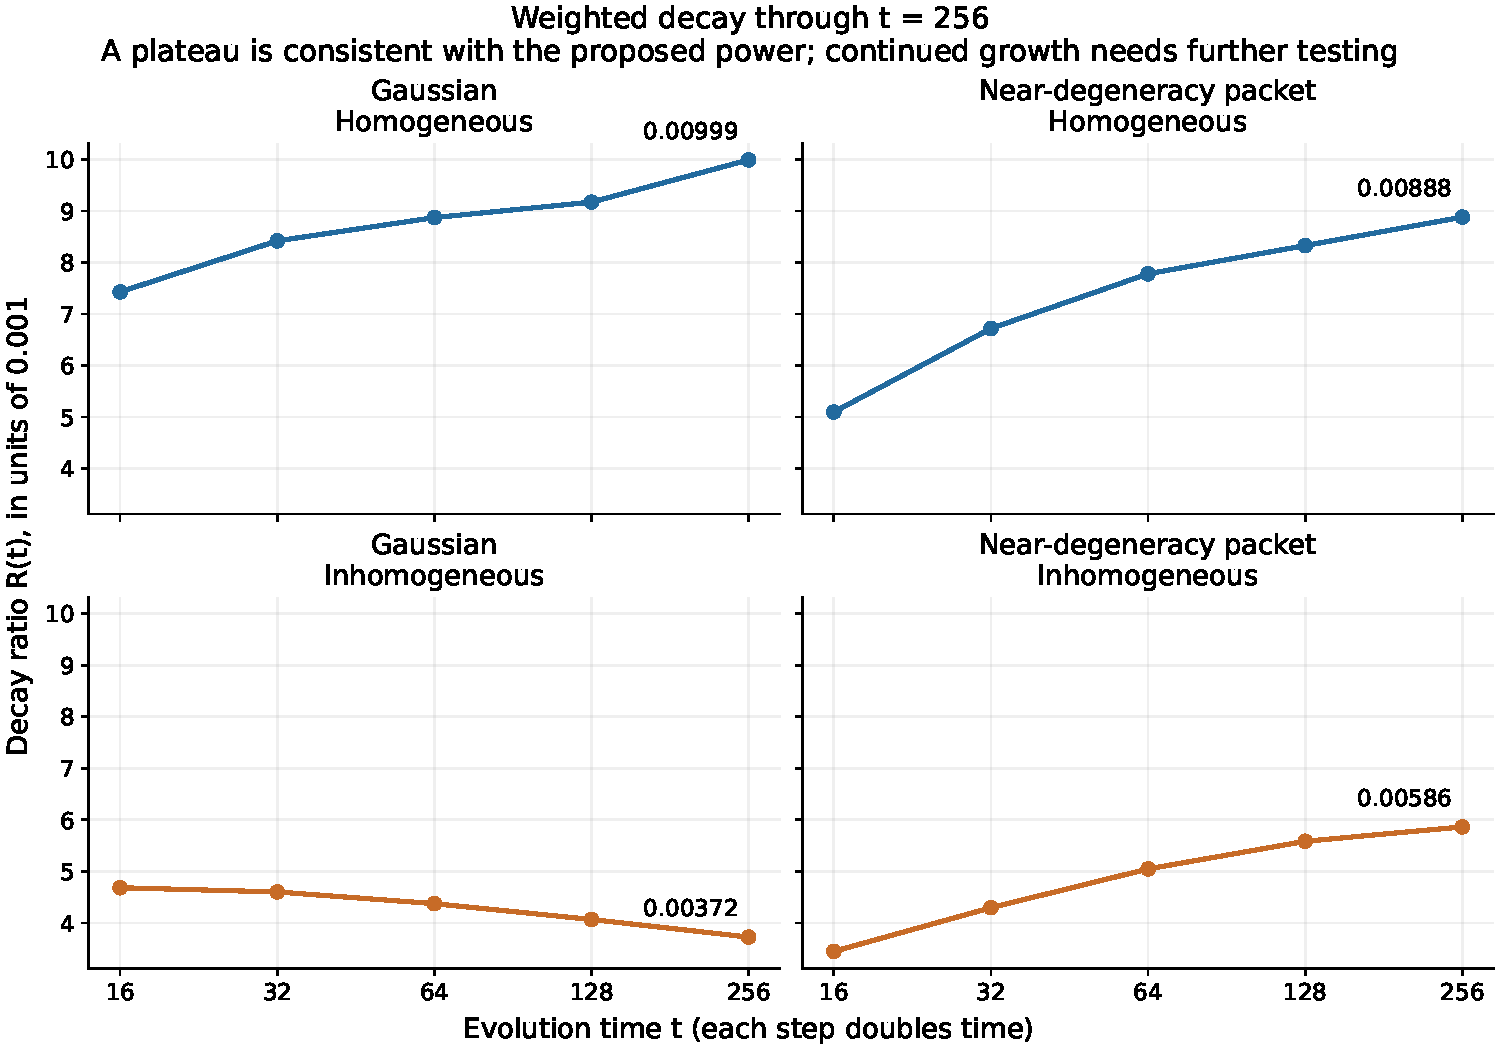
\includegraphics[width=\linewidth]{../results/long_time/decay_256.pdf}\end{center}
\textbf{Figure 3.} One curve per panel, with time doubling at each marker.
The ordinate is the same ratio $R(t)$ as before, displayed in units of $0.001$;
endpoint labels give its unscaled value. A downward curve means faster weighted
decay than $t^{-7/6}$ over that interval. An upward curve can still approach a
finite limit and does not by itself contradict the inequality.

\begin{center}\small
\begin{tabular}{llrrr}\toprule
Equation & Input & $R(128)$ & $R(256)$ & Effective exponent\\\midrule
\LongRows
\bottomrule\end{tabular}\end{center}
For weighted maximum $M(t)$, the last column is
$\gamma_{128,256}=-\log[M(256)/M(128)]/\log2$. It describes only the last time
doubling; it is not a fitted asymptotic exponent or a new uniform bound. The
paper's comparison exponent at $\alpha=1/2$ is $7/6\simeq1.167$.

\textbf{Finding.} The inhomogeneous Gaussian ratio decreases at late times.
The other three ratios increase over the last doubling, by different amounts.
None of these finite curves establishes a counterexample. The next question is
whether the rising ratios approach a finite limit or continue growing through
successive, independently checked time doublings.

\newpage
\section*{How the long-time calculation is checked}
Let $r=\sqrt{y^2+z^2}$ and use the exactly $L^1$-normalized initial profile
\[
 f(x,r)=\frac{\exp[-x^2/(2\sigma_x^2)-r^2/(2\sigma_y^2)]e^{iqx}}
 {(2\pi)^{3/2}\sigma_x\sigma_y^2}.
\]
The Gaussian has $(\sigma_x,\sigma_y,q)=(3,3,0)$; the near-degeneracy packet
has $(6,3,-\beta)$. Analytically integrating both transverse Fourier variables
reduces the weighted field to
\[
 W(x,r,t)=\frac1{4\pi^2}\int_{\mathbb R}
 \frac{|k+\beta|^{1/2}}{d(k,t)}
 \exp\!\left[-\frac{\sigma_x^2(k-q)^2}{2}+i(tk^3+kx)
             -\frac{r^2}{2d(k,t)}\right]dk,
 \qquad d(k,t)=\sigma_y^2-6it(sk+\beta).
\]
This is the same three-coordinate linear solution for these inputs. Only the
evaluation method changes. The transverse directions are treated on the whole
space; a longitudinal FFT quadrature evaluates many $x$ locations efficiently.
Radial symmetry reduces the spatial peak search to $(x,r)$.

\begin{center}\begin{tabular}{lrrrr}\toprule
Check & $x$ period & $\Delta x$ & Max. $r$ & $\Delta r$\\\midrule
Base & 4096 & 0.5 & 512 & 4\\
Expanded & 8192 & 0.5 & 1024 & 4\\
Refined & 8192 & 0.25 & 1024 & 2\\
Extra expansion at $t=256$ & 32768 & 0.25 & 2048 & 2\\\bottomrule
\end{tabular}\end{center}
The full $(x,r)$ search is followed by local optimization of the peak. At $256$,
the extra expansion changes the sampled peak by at most \LongDomain. An independent
adaptive quadrature of the integral above agrees with the complex field at each
final candidate peak to within \LongQuad\ relative error. The largest sampled
search-boundary amplitude is \LongEdge\ of its case's peak. These checks are
numerical evidence, not a certification that no larger unsampled peak exists.

\textbf{Why the previous box was inadequate.} At $t=256$, the inhomogeneous
near-degeneracy maximum lies around $x=-841$. It would be outside even the
length-288 box used for the earlier $t\le16$ runs. Extending time without changing
the spatial computation would therefore be unreliable.

\textbf{Remaining limits.} The Gaussian-specific reduction cannot be applied
unchanged to arbitrary measured fields or every artificial recipe. The adaptive
quadrature checks selected peak locations; the global search remains finite and
sampled. The two-dimensional radial search, local optimizer status, boundary ratios,
and domain/resolution comparisons are all recorded to make these limits reviewable.

\textbf{Reproduce.} Run \texttt{python3 long\_time\_decay.py}, followed by
\texttt{python3 report/make\_long\_time\_tables.py}. Results and the graph are under
\texttt{results/long\_time/}; compile \texttt{report/decay\_refinement.tex} for this
updated supplement. Source: the same manuscript, canonical symbols (6.2) and
weighted estimates in Propositions 6.2--6.3.
